\chapter{The PyBayes Library}

Introduction, general directions, future considerations

+ open development on github, open-source

\section{Interpreted and Compiled}

\section{Library Layout}

\begin{figure}[h]
	\centering
	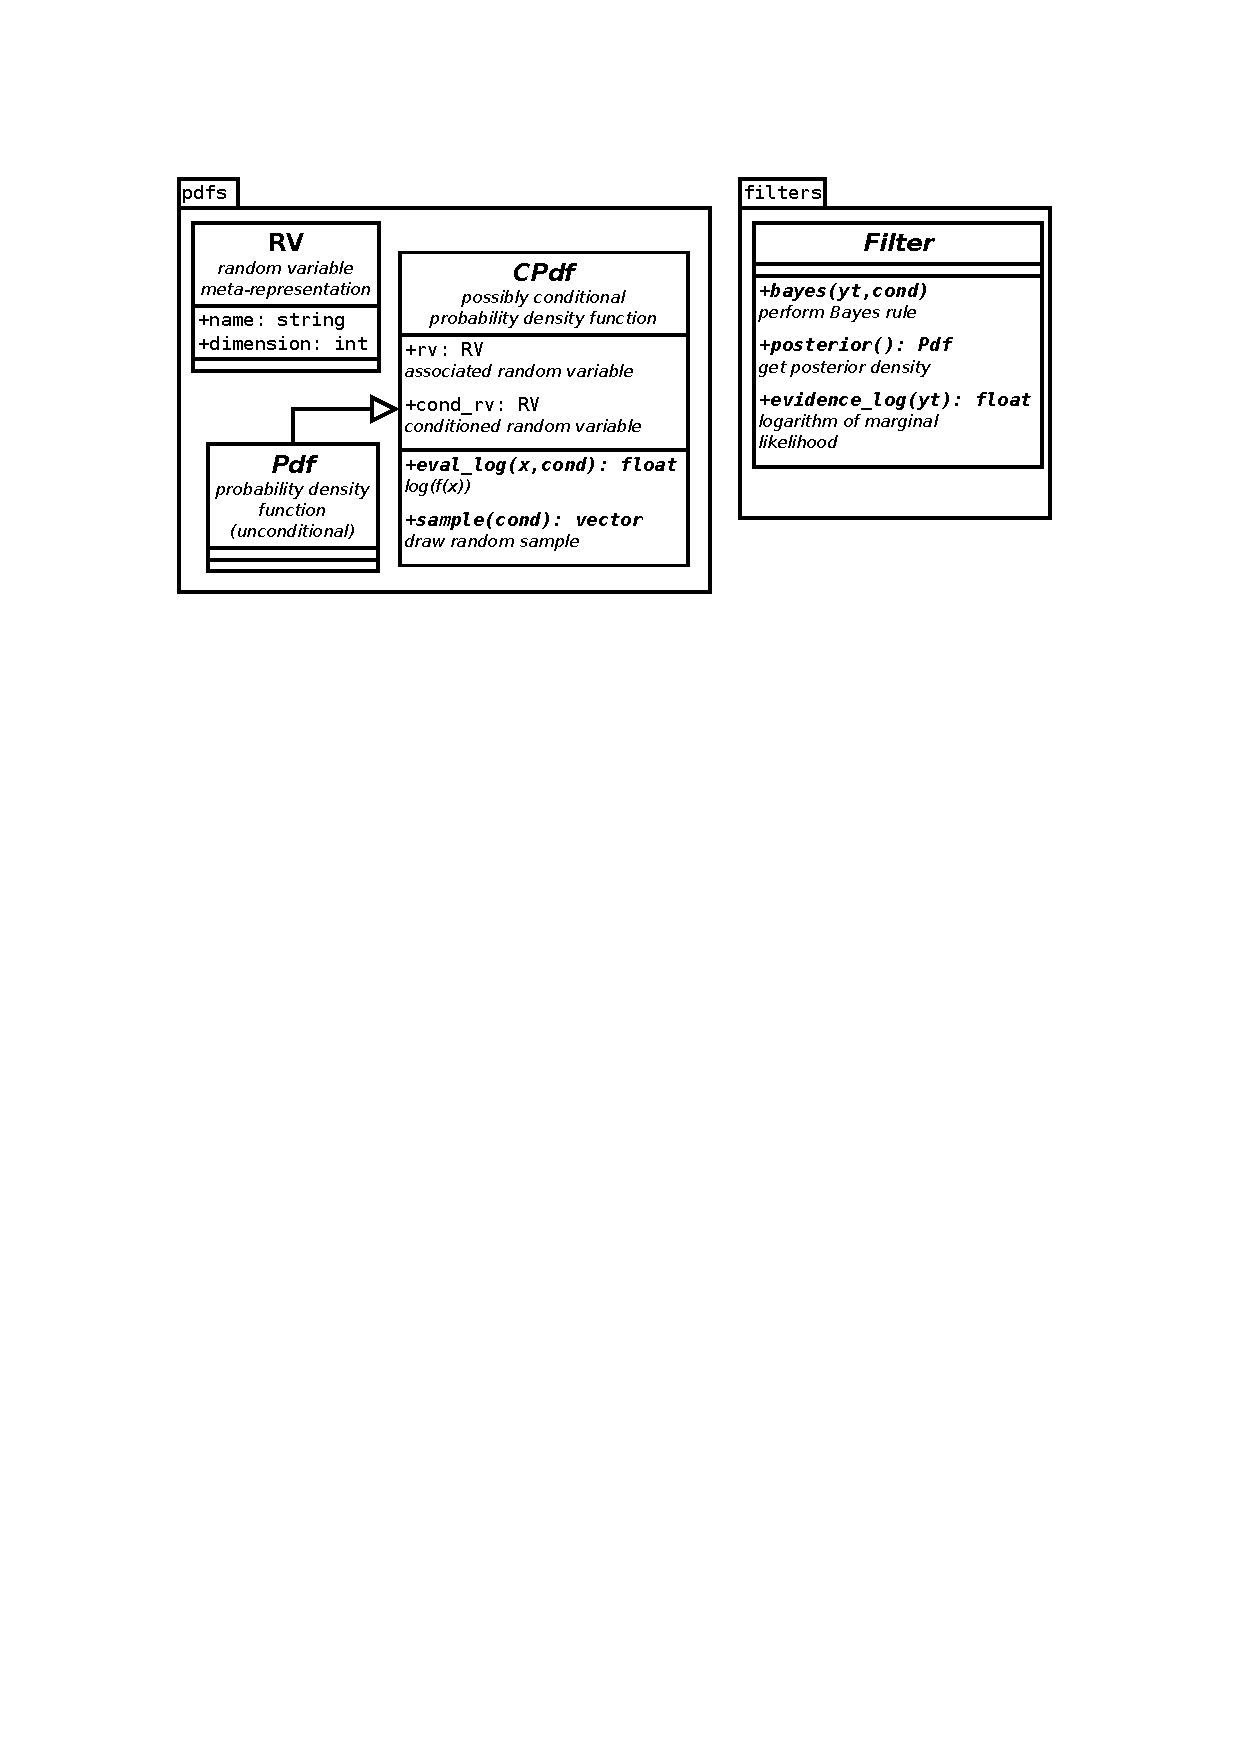
\includegraphics[width=\textwidth,keepaspectratio=true,clip=true,trim=3cm 196mm 3cm 3cm]{./diagrams/PyBayes.pdf}
	\vspace{-8mm}
	\caption{High-level overview of the PyBayes library; simplified}
\end{figure}

\subsection{Random Variable Meta-representation}

\begin{figure}[h]
	\centering
	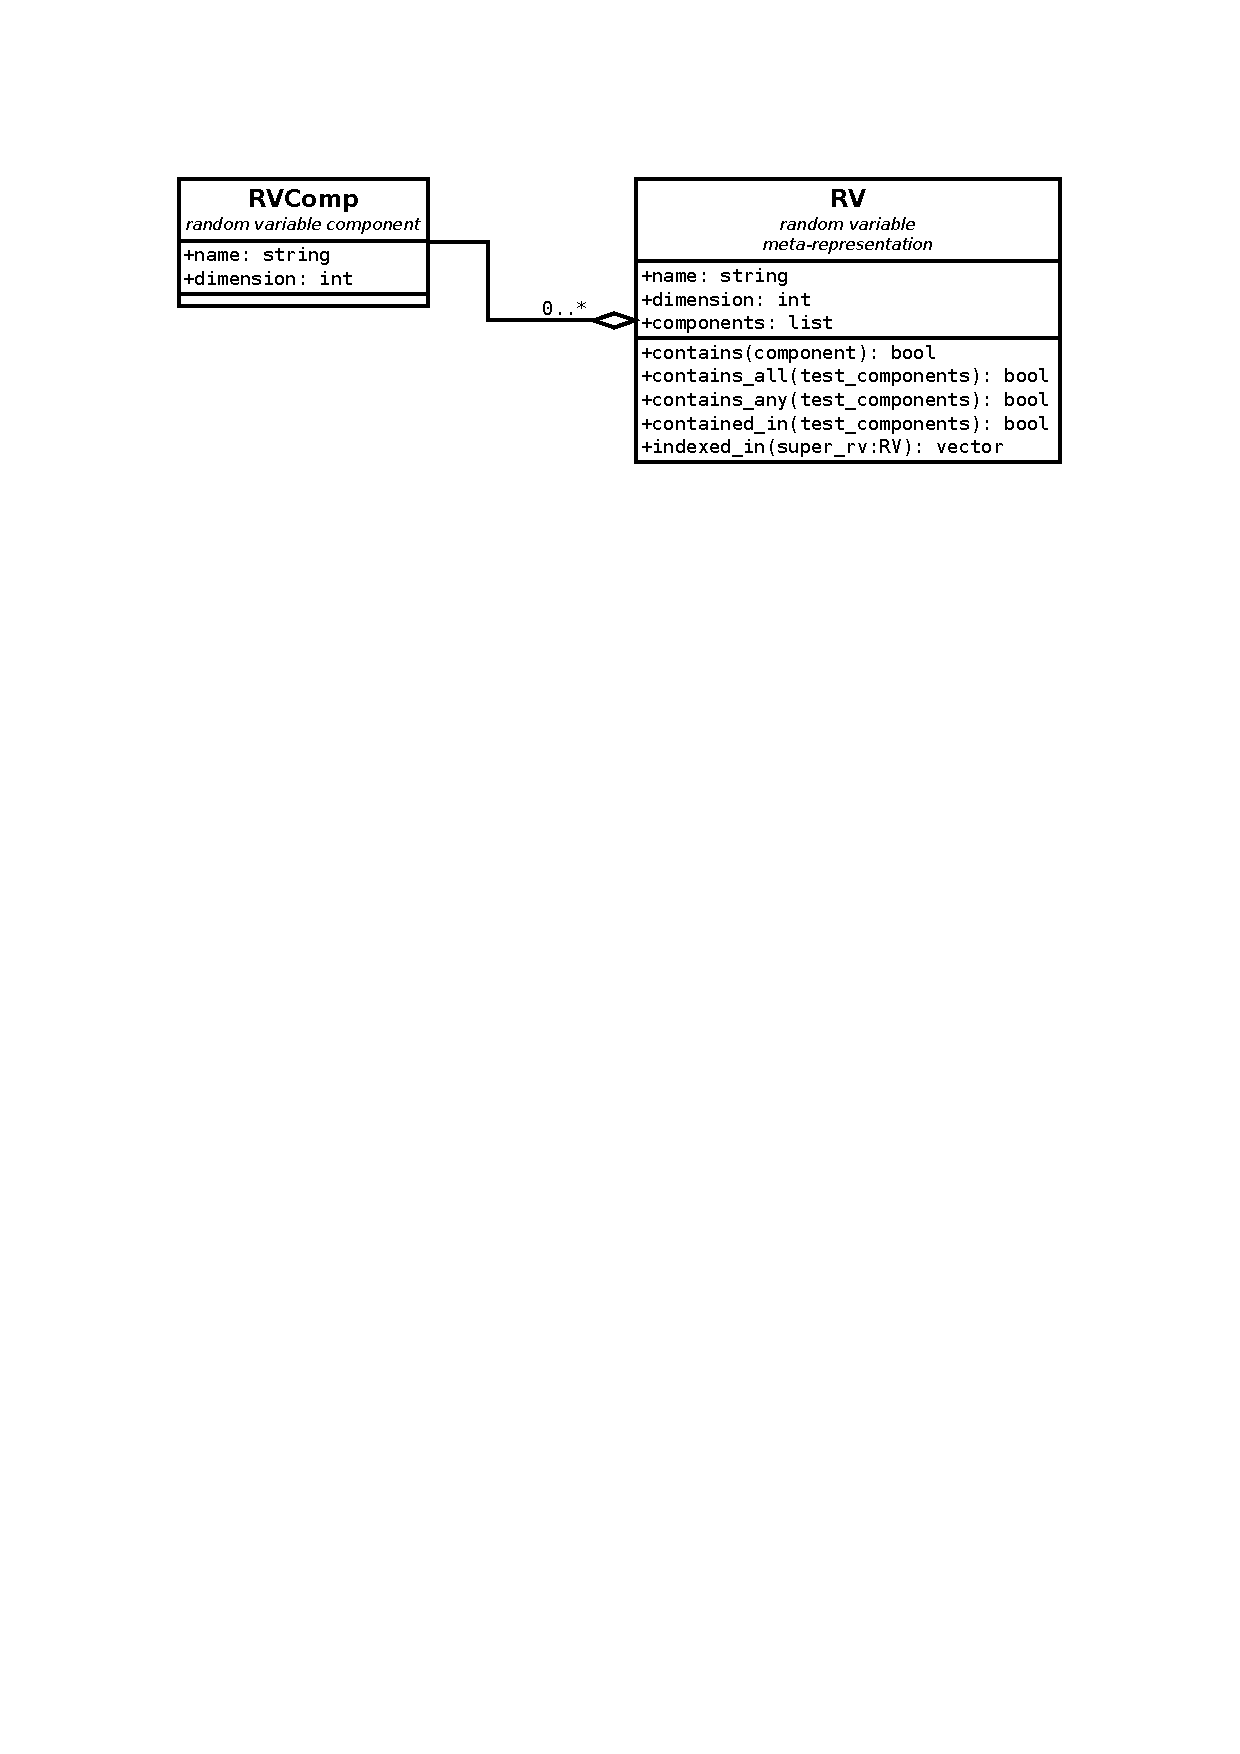
\includegraphics[width=\textwidth,keepaspectratio=true,clip=true,trim=3cm 218mm 3cm 3cm]{./diagrams/rvs.pdf}
	\vspace{-8mm}
	\caption{Class diagram of the random variable framework}
\end{figure}

Why it is needed (ref to ProdCPdf)

\subsection{Probability Density Functions}

\begin{figure}[h]
	\centering
	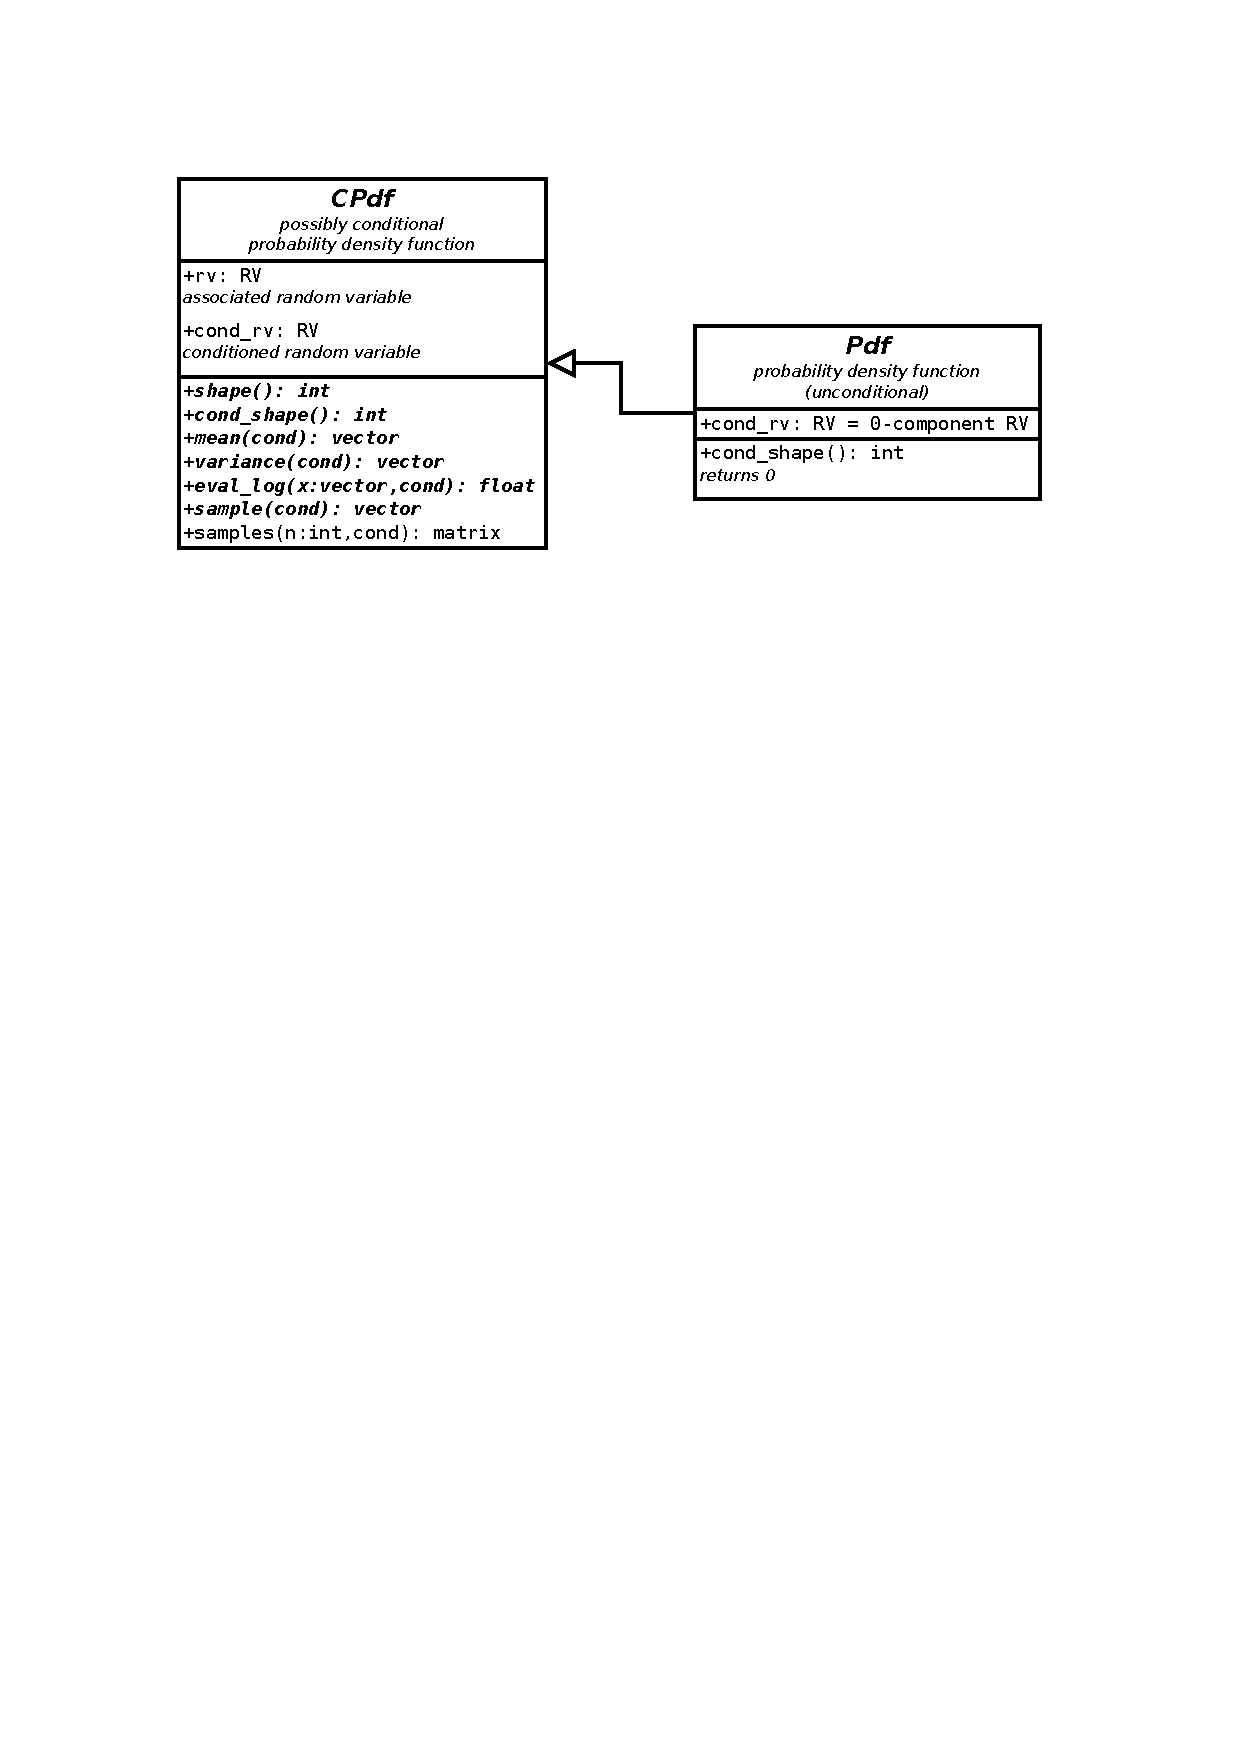
\includegraphics[width=\textwidth,keepaspectratio=true,clip=true,trim=3cm 204mm 3cm 3cm]{./diagrams/pdfs.pdf}
	\vspace{-8mm}
	\caption{Class diagram of the {\pdf} prototypes}
\end{figure}

Nice UML diagrams! (better more smaller UMLs than one big) One for general pdf layut, one for
AbstractGaussPdf family, one for AbstractEmpPdf family

\subsection{Bayesian Filters}

[proposed citation: \cite{Smi:05}]

UML

Nice graph of a run of a particle filter (Mirda has the plotting code)

similar of marginalized particle filter? (gausses would be plotted vertically)

[mention this:\cite{Smi:10}]

\section{Documentation, Testing and Profiling} \label{sec:PyBayesDocsTests}

TODO: move above Library Layout?

Documenting PyBayes using Sphinx, approach to documentation (mathematician-oriented), math in documentation

Testing - the separation of

- tests: test one class in isolation, quick, determinism (would be good, not achievable)

- stresses: test a great portion of code at once, run longer, non-determinism..

Note about coverage.py!!

Profiling python/cython - how, existing support in PyBayes

- how to correct profiling-induced overhead

\section{Performance Comparison with BDM} \label{sec:PyBayesPerformance}

[skip if in time press]
